\documentclass[12pt]{article}
\usepackage[utf8]{inputenc}
\usepackage[russian]{babel}
\usepackage{graphicx}
\usepackage{listings}
\usepackage{indentfirst}
\usepackage{color}
\usepackage{bm}

\definecolor{dkgreen}{rgb}{0,0.6,0}
\definecolor{gray}{rgb}{0.5,0.5,0.5}
\definecolor{ltgray}{rgb}{0.95,0.95,0.95}
\definecolor{mauve}{rgb}{0.58,0,0.82}
\newcommand{\rot}{\mathop{\rm rot}\nolimits}
\renewcommand{\lstlistingname}{Листинг}
\lstset{ %
  language=Python,                % the language of the code
  basicstyle=\footnotesize\ttfamily,           % the size of the fonts that are used for the code
%  numbers=left,                   % where to put the line-numbers
%  numberstyle=\tiny\color{gray},  % the style that is used for the line-numbers
%  stepnumber=2,                   % the step between two line-numbers. If it's 1, each line 
                                  % will be numbered
%  numbersep=5pt,                  % how far the line-numbers are from the code
  backgroundcolor=\color{ltgray},      % choose the background color. You must add \usepackage{color}
  showspaces=false,               % show spaces adding particular underscores
  showstringspaces=false,         % underline spaces within strings
  showtabs=false,                 % show tabs within strings adding particular underscores
  %frame=single,                   % adds a frame around the code
  rulecolor=\color{black},        % if not set, the frame-color may be changed on line-breaks within not-black text (e.g. comments (green here))
  columns=fixed,
  tabsize=2,                      % sets default tabsize to 2 spaces
  captionpos=b,                   % sets the caption-position to bottom
  breaklines=true,                % sets automatic line breaking
  breakatwhitespace=false,        % sets if automatic breaks should only happen at whitespace
%  caption=Valalala,                   % show the filename of files included with \lstinputlisting;
                                  % also try caption instead of title
  keywordstyle=\color{blue},          % keyword style
  commentstyle=\color{gray},       % comment style
  stringstyle=\color{dkgreen},         % string literal style
  escapeinside={\%*}{*)},            % if you want to add LaTeX within your code
  morekeywords={*,...},              % if you want to add more keywords to the set
  deletekeywords={...}              % if you want to delete keywords from the given language
}


\title{Сравнительное использование конечных элементов для стационарной задачи о течении в каверне с подвижной верхней границей}
\author{Виктор Борисов}

\begin{document}

\maketitle

\section{Задача о течении в каверне}
Стационарные уравнения Стокса описывают устоявшееся несжимаемое течение в области $\Omega$ с границей $\Gamma$
\begin{equation}
-\Delta {\bm u} + \nabla p = {\bm f}, \quad {\bm x} \in \Omega,
\end{equation}
\begin{equation}
\nabla\cdot{\bm u} = {\bm 0}, \quad {\bm x} \in \Omega,
\end{equation}
\begin{equation}
{\bm u} = {\bm g}, \quad {\bm x} \in \Gamma,
\end{equation}
где $\bm u$ - скорость, $p$ - давление и $\bm f$ - внутренний источник движения. В двумерной задаче ${\bm x}=(x_1, x_2)$, остальные векторные величины задаются аналогично.
В этой постановке присутствуют две зависимые неизвестные: скорость и давление.
В численном решении этого и вообще всех уравнений типа Навье-Стокса, используемые конечные элементы должны удовлетворять условию Ладыженской-Бабушки-Бреззи. Часто используемые полиномы Лагранжа второго порядка для давления и скорости приводят к несходимости решения.

В качестве тестовой задачи рассматривается двумерная задача о течении в каверне с подвижной верхней границей. Подвижная верхняя граница означает, что вектор скорости имеет ненулевое значение на ней. Постановка и решение тестовой задачи не имеют физических единиц измерения. Мы рассматриваем единичный квадрат $\Omega$ (рис. \ref{fg:cavity}), c границей $\Gamma=\Gamma_1 \cup \Gamma_2$, где на верхней границе $\Gamma_1$ скорость принимает значения $u_1=1$ и $u_2=0$, в остальной части $\Gamma_2$ поставлено условие неприлипания ${\bm u}={\bm 0}$.

\begin{figure}
	\begin{center}
		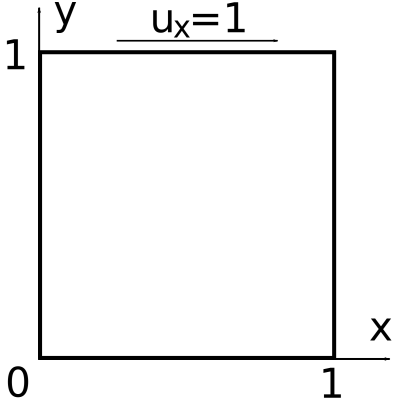
\includegraphics[width=200px]{pics/cavity400}
		\caption{Тестовая область с подвижной верхней границей.}
		\label{fg:cavity}
	\end{center}
\end{figure}

\section{Конечные элементы}
Для численного решения методом конечных элементов, для начала систему уравнений переписывают в вариационную постановку:
\begin{equation}
a(u,v)-b(v,p)=(f,v) \quad \forall v \in V,
\end{equation}
\begin{equation}
b(u,q)=0 \quad \forall q \in \Pi,
\end{equation}
где 
\begin{equation}
a(u,v)=\int_\Omega \nabla v \cdot \nabla v \, dx,
\end{equation}
\begin{equation}
b(v,q)=\int_\Omega (\nabla \cdot v) q \, dx,
\end{equation}
\begin{equation}
(f,v)=\int_\Omega f \cdot v \, dx.
\end{equation}
В этой постановке множества $V$ и $\Pi$ это функциональные пространства для скорости и давления соответственно. Эти пространства определяются из конечных элементов, выбор которых влияет на качества решения. Рассматриваются три набора элементов: Taylor Hood (TH), continious discontinious Lagrange (CD), Crouzeix Raviart (CR). 

Набор TH состоит из двух полиномов Лагранжа (Lagrange) для скорости и давления. Причем порядок полинома для скорости на единицы выше чем для давления. На рис. \ref{fg:lagrange2} элемент второго порядка, для первого порядка исчезают точки по середине сторон треугольника.

Набор CD состоит из полиномов Лагранжа порядка 2 для скорости и разрывного элемента Лагранжа (Discontinuous Lagrange) порядка 0.

Набор CR это элемент Crouzeix Raviart для скорости и разрывный элемент Лагранжа порядка 0 для давления. На рис. \ref{fg:crouzeix1} представлен элемент первого порядка. Точки определяющие степени свободы расположены не на концах треугольника, а на середине сторон.

Набор TH и CD имеют максимум второй порядок, а CR первый, что будет сказываться на свойствах решения.

\begin{figure}
	\begin{center}
		\includegraphics[width=200px]{pics/lagrange2}
		\caption{Элемент Лагранжа второго порядка.}
		\label{fg:lagrange2}
	\end{center}
\end{figure}

\begin{figure}
	\begin{center}
		\includegraphics[width=200px]{pics/crouzeix1}
		\caption{Элемент Crouzeix Raviart первого порядка.}
		\label{fg:crouzeix1}
	\end{center}
\end{figure}

\section{Решение}
В данном разделе описывается используемый способ сравнения решений полученных с помощью различных наборов конечных элементов. Используется функция тока, как показатель решения двумерной задачи с вычислением поля скоростей. Приводится отрывок из программы на языке Python с использованием библиотеки Fenics.

\subsection{Сравнение сходимости решения}
Сравнение должно происходить с точным решением, но его у нас нет. Поэтому <<точным>> решением будем считать результат полученный на мелкой сетке. Все выбранные наборы элементов должны сходиться к этому решению при измельчении сетки. Исходная область (единичный квадрат) делиться на $N^2$ квадратов, и каждый квадрат делится на два треугольника. $N$ будем считать размером сетки.

Сравнить сходимость на разных сетках будем с результатом полученным на сетке размером $N=200$ с использованием набора TH. 

\subsection{Функция тока}
В задачах с вычислением вектора скорости одним из общепринятых показателей является функция тока. Визуальное сравнение множества двумерных векторов скорости не очевидно, поэтому вместо двумерных векторов скорости - сравнивают скалярную функцию тока. Функция тока обладает следующими свойствами:
\begin{equation}
u_x = \frac{\partial \psi}{\partial y},
\end{equation}
\begin{equation}
u_y = - \frac{\partial \psi}{\partial x}.
\end{equation}
Чтобы вычислить $\psi$, надо решить уравнение Лапласа:
\begin{equation}
\Delta\psi=-\xi,
\end{equation}
где $\rot {\bm u} = (0, 0, \xi)$.

\subsection{Сравниваемые свойства результатов}
Вычисляются решения на разных сетках, изменяя параметр $N$ и наборы конечных элементов указанных выше.
Нас интересует время и погрешность вычисления решения.

Время вычисления $t_N$ это количество времени потраченное на решение общей системы линейных уравнений.

Погрешность вычисления скорости $\bm u_{err}$ это разница между текущим решением $\bm u_N$ и решением на мелкой сетке $\bm u_{ex}$
\begin{equation}
{\bm r_{u}} = {\bm u_{ex}} - {\bm u_N}.
\end{equation}
Для сравнения, берем норму погрешности $u_{err}$ в пространстве $L_2$
\begin{equation}
||u_{err}||^2 = \int_{\Omega} {\bm r_{u}}^2 dx.
\end{equation}
Погрешности для давления и функции тока вычисляются аналогично.

\subsection{Программа}
Программа составлена на языке Python с помощью библиотеки Fenics.
Основные параметры программы это наборы элементов:
\begin{lstlisting}
elements_table = {
    "CR": ("Crouzeix-Raviart", 1, 
                          "Discontinuous Lagrange", 0),
    "CD": ("Lagrange", 2, "Discontinuous Lagrange", 0),    
    "TH": ("Lagrange", 2, "Lagrange", 1),
}
\end{lstlisting}
где каждый набор это название элемента для скорости, порядок элемента для скорости, название элемента для давления и порядок элемента для давления. Также основными параметрами являются размеры сетки:
\begin{lstlisting}
n_min = 25  # minimum size
n_max = 200 # maximum size
h     = 5   # step size
\end{lstlisting}

Возможности библиотеки Fenics позволяют довольно просто составлять процедуры решения вычислительной задачи. Сетка это единичный квадрат с $N^2$ узлами:
\begin{lstlisting}
def create_mesh(n):
    mesh = UnitSquare(n, n)
    return mesh
\end{lstlisting}

Создание функциональных пространств, элемент и его порядок берутся из таблицы elements\_table:
\begin{lstlisting}
def create_space(element, mesh):
    (u_element, u_order, p_element, p_order) = main.elements_table[element]
    U = VectorFunctionSpace(mesh, u_element, u_order)
    P = FunctionSpace(mesh, p_element, p_order)
    W = U*P
    return W
\end{lstlisting}

Процедура решения задачи о течении в каверне: 
\begin{lstlisting}       
def solve_cavity(mesh, space):
    def domain_top(x, on_boundary):
        return on_boundary and x[1] > 1 - DOLFIN_EPS  
    def domain_walls(x, on_boundary):
        return on_boundary and x[1] < 1 - DOLFIN_EPS    
    bc0 = DirichletBC(space.sub(0), Constant((0,0)), domain_walls)
    bc1 = DirichletBC(space.sub(0), Constant((1,0)), domain_top)
    bcs = [bc0, bc1]    
    (u, p) = TrialFunctions(space)
    (v, q) = TestFunctions(space)
    f = Constant((0, 0))       
    a = inner(grad(u), grad(v))*dx - p*div(v)*dx + div(u)*q*dx
    L = inner(f, v)*dx    
    t = Timer("Solve timing");
    t.start()            
    U = Function(space)
    problem = LinearVariationalProblem(a, L, U, bcs=bcs)
    solver = LinearVariationalSolver(problem)
    solver.solve()    
    t.stop()    
    (u, p) = U.split(True)        
    # correct pressure
    c = assemble(p*dx)
    vec = p.vector()
    for i in range(vec.size()):
        vec[i] -= c
    return u, p, t.value()
\end{lstlisting}
Вложенные процедуры domain\_top и domain\_walls описывают верхнюю подвижную границу $\Gamma_1$, и неподвижную границу $\Gamma_2$ соответственно. После вычисления идет поправка давления, т.к. давление вычисляется с точностью до константы.

Процедура вычисления функции тока $\psi$:
\begin{lstlisting}
def solve_cavity_psi(mesh, space, u):
    V = FunctionSpace(mesh, "Lagrange", 2)
    def domain_walls(x, on_boundary):
        return on_boundary
    bc1 = DirichletBC(V, Constant(0), domain_walls)    
    bcs = [bc1]
    psi = TrialFunction(V)
    v = TestFunction(V)    
    a = inner(grad(psi), grad(v))*dx
    L = inner(-rot(u), v)*dx    
    PSI = Function(V)
    problem = LinearVariationalProblem(a, L, PSI, bcs=bcs)
    solver = LinearVariationalSolver(problem)
    solver.solve()
    return PSI
\end{lstlisting}

Процедура вычисления погрешности решения:
\begin{lstlisting}
def solve_cavity_error(u,    p,    psi,    
                       u_ex, p_ex, psi_ex, mesh_ex):
    M = inner((u_ex - u),(u_ex - u))*dx
    v_err = assemble(M, mesh=mesh_ex)    
    Mp = (p_ex - p)*(p_ex - p)*dx
    p_err = assemble(Mp, mesh=mesh_ex)
    Mps = (psi_ex - psi)*(psi_ex - psi)*dx
    psi_err = assemble(Mps, mesh=mesh_ex)
    return (v_err, p_err, psi_err)
\end{lstlisting}
Происходит сравнение с точными решениями ${\bm u_{ex}}$, $p_{ex}$ и $\psi_{ex}$.

\section{Результаты}
В результате вычисления получаем функции u, p, psi определенные на выбранных наборах конечных элементов и сетки. Естественно, что на более грубой сетки вычисляемое значения функции интерполируется если не попадает в узел. Для сравнения результатов, вычисляются значения на этих функциях во всех значениях сетки mesh\_ex, и сохраняются в файле.

\subsection{Графики}
\begin{figure}
	\begin{center}
		\includegraphics[width=400px]{pics/time}
		\caption{Зависимость времени вычисления от размера области для наборов элементов CR, TH, CD.}
		\label{fg:time}
	\end{center}
\end{figure}

\begin{figure}
	\begin{center}
		\includegraphics[width=400px]{pics/u_err}
		\caption{Зависимость погрешности скорости от размера области для наборов элементов CR, TH, CD.}
		\label{fg:u_err}
	\end{center}
\end{figure}

\begin{figure}
	\begin{center}
		\includegraphics[width=400px]{pics/p_err}
		\caption{Зависимость погрешности давления от размера области для наборов элементов CR, TH, CD.}
		\label{fg:p_err}
	\end{center}
\end{figure}

\begin{figure}
	\begin{center}
		\includegraphics[width=400px]{pics/psi_err}
		\caption{Зависимость погрешности функции тока от размера области для наборов элементов CR, TH, CD.}
		\label{fg:psi_err}
	\end{center}
\end{figure}

\begin{figure}
	\begin{center}
		\includegraphics[width=400px]{pics/psi_25}
		\caption{Функция тока на разрезе по $x=0.5$ при $N=25$ для наборов элементов CR, TH, CD. Линия EX - точное решение.}
		\label{fg:psi_25}
	\end{center}
\end{figure}

\begin{figure}
	\begin{center}
		\includegraphics[width=400px]{pics/psi_50}
		\caption{Функция тока на разрезе по $x=0.5$ при $N=50$ для наборов элементов CR, TH, CD. Линия EX - точное решение.}
		\label{fg:psi_50}
	\end{center}
\end{figure}

\begin{figure}
	\begin{center}
		\includegraphics[width=400px]{pics/psi_100}
		\caption{Функция тока на разрезе по $x=0.5$ при $N=100$ для наборов элементов CR, TH, CD. Линия EX - точное решение.}
		\label{fg:psi_100}
	\end{center}
\end{figure}

\begin{figure}
	\begin{center}
		\includegraphics[width=400px]{pics/psi_150}
		\caption{Функция тока на разрезе по $x=0.5$ при $N=150$ для наборов элементов CR, TH, CD. Линия EX - точное решение.}
		\label{fg:psi_150}
	\end{center}
\end{figure}

\newpage
\subsection{Выводы}
Применять только наборы элементов Taylor-Hood. Они супер-круты.

\end{document}